Partendo dalle architetture utilizzate nel progetto di riferimento, ne sono state ricercate di migliori per il task in questione. Nello specifico le architetture di cui si è testata l'efficacia sono le seguenti: 

\begin{itemize}
    \item Random Forest
    \item Rete neurale
    \item Reti neurali ricorrenti (con layer Keras come LSTM e GRU)
\end{itemize}

Di seguito queste architetture verranno elencate mostrando i dettagli relativi ai layer che le compongone e le relative prestazioni.

\subsection{Random forest}
Per quanto riguarda i Random Forest sono stati inizialmente utilizzati solo due stimatori, ma senza ottenere buone prestazioni. Quindi, è stato introdotto l'utilizzo di una Grid Search con cui sono stati ottenuti i valori migliori circa il numero di stimatori, il random state ed, infine, il max depth:

\begin{table}[h]
    \centering
    \begin{tabular}{|c|c|c|}
    \hline
         Numero stimatori & Random state & Max depth\\
    \hline
        1 & 1 & 3 \\
    \hline
    \end{tabular}
    \caption{Parametri migliori per il Random Forest}
    \label{tab:rdmF_bestParams}
\end{table}

\begin{table}[h]
    \centering
    \begin{tabular}{|c|c|}
    \hline
         & Score \\
         \hline
         Training & 0.42894736842105263 \\
         \hline
         Test & 0.41842105263157897 \\
    \hline
    \end{tabular}
    \caption{Prestazioni ottenute con i parametri in tabella~\ref{tab:rdmF_bestParams}}
    \label{tab:my_label}
\end{table}

\newpage
\subsection{Rete neurale}
Un'ulteriore tecnica di Machine Learning ha previsto l'uso di una rete neurale con layer \textit{Fully Connected} con attivazione di tipo \textbf{\textit{relu}} (ad eccezione dell'ultimo con attivazione \textbf{\textit{softmax}}) e l'utilizzo di \textit{Dropout} caratterizzata come segue:
% \newpage
\begin{lstlisting}[style=arch]
Model: "sequential_1"
_________________________________________________________________
Layer (type)                 Output Shape              Param #   
=================================================================
flatten_1 (Flatten)          (3135, 94)                0         
_________________________________________________________________
dense_3 (Dense)              (3135, 300)               28500     
_________________________________________________________________
dense_4 (Dense)              (3135, 100)               30100     
_________________________________________________________________
dropout_1 (Dropout)          (3135, 100)               0         
_________________________________________________________________
dense_5 (Dense)              (3135, 3)                 303       
=================================================================
Total params: 58,903
Trainable params: 58,903
Non-trainable params: 0
_________________________________________________________________
\end{lstlisting}
\begin{lstlisting}[style=report]
TRAIN REPORT
              precision    recall  f1-score   support

           A      0.402     0.905     0.557       896
           D      0.000     0.000     0.000       809
           H      0.735     0.575     0.645      1430

    accuracy                          0.521      3135
   macro avg      0.379     0.493     0.401      3135
weighted avg      0.450     0.521     0.453      3135

--------------------------------------------------
TEST REPORT
              precision    recall  f1-score   support

           A      0.420     0.908     0.575       316
           D      0.000     0.000     0.000       228
           H      0.740     0.535     0.621       501

    accuracy                          0.531      1045
   macro avg      0.387     0.481     0.399      1045
weighted avg      0.482     0.531     0.472      1045

--------------------------------------------------
\end{lstlisting}

\subsection{Reti neurali ricorrenti}\label{sec:rnn}
Per applicare l'uso delle architetture ricorrenti, in primo luogo è stato analizzato il dataset e, successivamente, è stato approfondito come i dati vengano ricevuti in input dall'\textit{LSTM} utilizzata nel progetto di riferimento. Di conseguenza, sono stati decisi ed adottati due approcci differenti, accumunati dall'idea di dividere il dataset in sequenze di $n$ partite, dove $n$ è un parametro che è stato fissato a $10$: nel primo approccio questa suddivisione è effettuata sul dataset iniziale, mentre nel secondo su un dataset generato, partendo da quello iniziale, collezionando ed ordinando cronologicamente tutte le partite di ogni singola squadra, che sono state poi concatenate.

Inoltre, a causa di tale eterogeneità nella rappresentazione dei dati nei due approcci, è stata introdotta una differenziazione anche relativamente alle architetture: nel primo caso il layer ricorrente agisce come una \textbf{\textit{sequence to sequence}}, predicendo tutte le partite della sequenza, mentre nel secondo come una \textbf{\textit{sequence to vector}} pronosticando esclusivamente il risultato dell'ultima in sequenza. 

In generale per ciascuna di queste architetture è stato seguito il medesimo approccio per cui ad uno o più layer ricorrenti iniziali sono stati concatenati strati \textit{Fully Connected} intervallati da \textit{Dropout}.

Infine, durante l'addestramento di ciascuna di queste architetture è stata introdotta la tecnica dell'\textbf{\textit{EarlyStopping}} per far in modo che la fase di training si concludesse una volta terminato l'apprendimento della rete, onde così evitare fenomeni di \textbf{\textit{overfitting}}.

\subsubsection*{SimpleRNN}
\begin{lstlisting}[style=arch]
Model: "sequential_1"
_________________________________________________________________
Layer (type)                 Output Shape              Param #   
=================================================================
simple_rnn (SimpleRNN)       (304, 10, 64)             10176     
_________________________________________________________________
dropout_3 (Dropout)          (304, 10, 64)             0         
_________________________________________________________________
dense_3 (Dense)              (304, 10, 1000)           65000     
_________________________________________________________________
dropout_4 (Dropout)          (304, 10, 1000)           0         
_________________________________________________________________
dense_4 (Dense)              (304, 10, 250)            250250    
_________________________________________________________________
dropout_5 (Dropout)          (304, 10, 250)            0         
_________________________________________________________________
dense_5 (Dense)              (304, 10, 3)              753       
=================================================================
Total params: 326,179
Trainable params: 326,179
Non-trainable params: 0
_________________________________________________________________
\end{lstlisting}
\begin{lstlisting}[style=report]
TRAIN REPORT
                precision   recall  f1-score    support
            A       0.527    0.611     0.566        867
            D       0.500    0.001     0.003        783
            H       0.590    0.863     0.701       1390

     accuracy                          0.569       3040
    macro avg       0.539    0.492     0.423       3040
 weighted avg       0.549    0.569     0.482       3040
 __________________________________________________
TEST REPORT
                precision   recall  f1-score    support
            A       0.579    0.672     0.622        345
            D       0.000    0.000     0.000        254
            H       0.609    0.832     0.703        541

     accuracy                          0.598       1140
    macro avg       0.392    0.501     0.442       1140
 weighted avg       0.464    0.598     0.522       1140
\end{lstlisting}


\subsubsection*{LSTM}
\begin{lstlisting}[style=arch]
Model: "sequential"
_________________________________________________________________
Layer (type)                 Output Shape              Param #   
=================================================================
lstm (LSTM)                  (304, 10, 64)             40704     
_________________________________________________________________
dropout (Dropout)            (304, 10, 64)             0         
_________________________________________________________________
dense (Dense)                (304, 10, 1000)           65000     
_________________________________________________________________
dropout_1 (Dropout)          (304, 10, 1000)           0         
_________________________________________________________________
dense_1 (Dense)              (304, 10, 250)            250250    
_________________________________________________________________
dropout_2 (Dropout)          (304, 10, 250)            0         
_________________________________________________________________
dense_2 (Dense)              (304, 10, 3)              753       
=================================================================
Total params: 356,707
...
Trainable params: 356,707
Non-trainable params: 0
_________________________________________________________________

\end{lstlisting}

\begin{lstlisting}[style=report]
TRAIN REPORT
                precision   recall  f1-score    support
            A       0.568    0.567     0.567        867
            D       0.506    0.109     0.179        783
            H       0.602    0.869     0.711       1390

     accuracy                          0.587       3040
    macro avg       0.558    0.515     0.486       3040
 weighted avg       0.567    0.587     0.533       3040
 __________________________________________________
TEST REPORT
                precision   recall  f1-score    support
            A       0.618    0.583     0.600        345
            D       0.348    0.122     0.181        254
            H       0.614    0.824     0.704        541

     accuracy                          0.595       1140
    macro avg       0.527    0.510     0.495       1140
 weighted avg       0.556    0.595     0.556       1140
\end{lstlisting}

Si è anche testata l'efficacia di più layer \textit{LSTM} concatenati o parallelizzati, ma in entrambi i casi le prestazioni non sono migliorate significativamente. 

Successivamente, oltre agli approcci precedentemente accennati, poiché non hanno introdotto miglioramenti nelle prestazioni, si è pensato di verificare se fosse vantaggioso un differente approccio: i \textit{time steps}, piuttosto che corrispondere a sequenze di $n$ partite, si potrebbero associare alla singola partita e farli coincidere a sequenze composte dalle features selezionate (vedi \cite{web:football_lstm}).

Si noti che questo approccio è stato utilizzato per la successiva architettura:

% \begin{figure}[h]
%       \begin{subcaptionblock}{.55\textwidth}
%         \centering
%         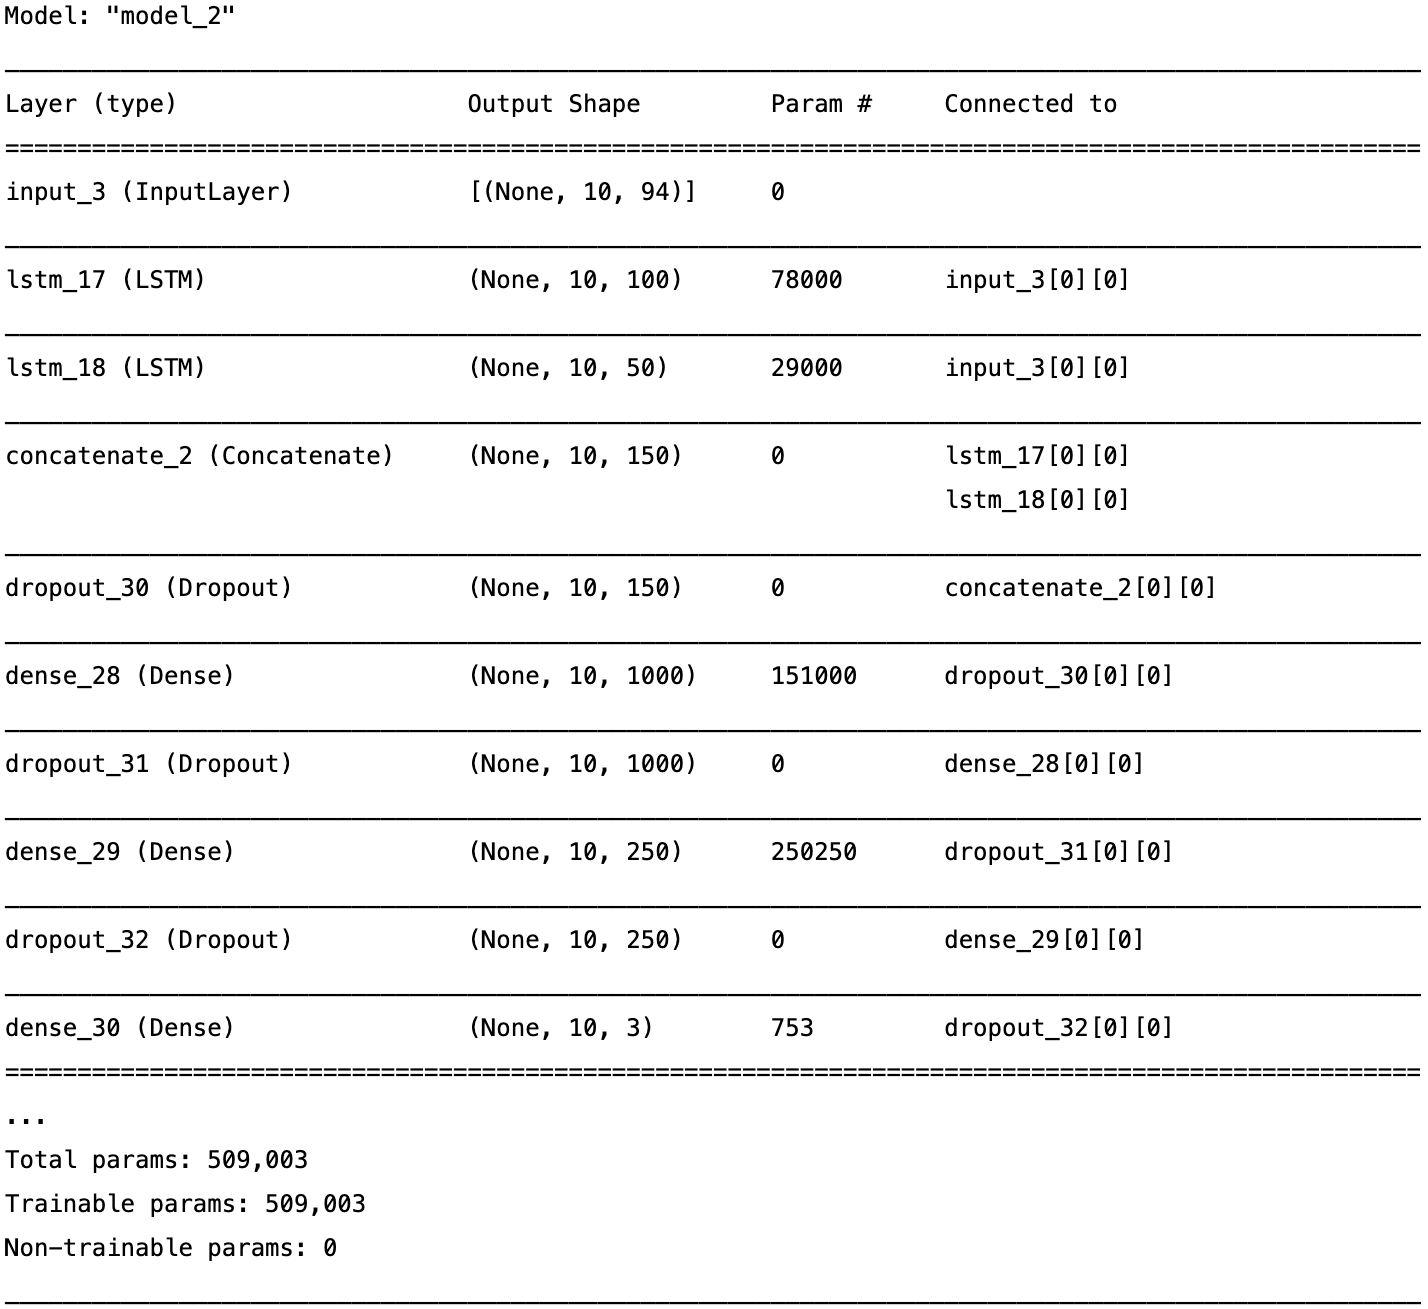
\includegraphics[scale=0.3]{tesina/img/lstm_concat/model_summary.png}
%       \end{subcaptionblock}
%       \begin{subcaptionblock}{.5\textwidth}
%         \begin{subcaptionblock}{.5\textwidth}
%             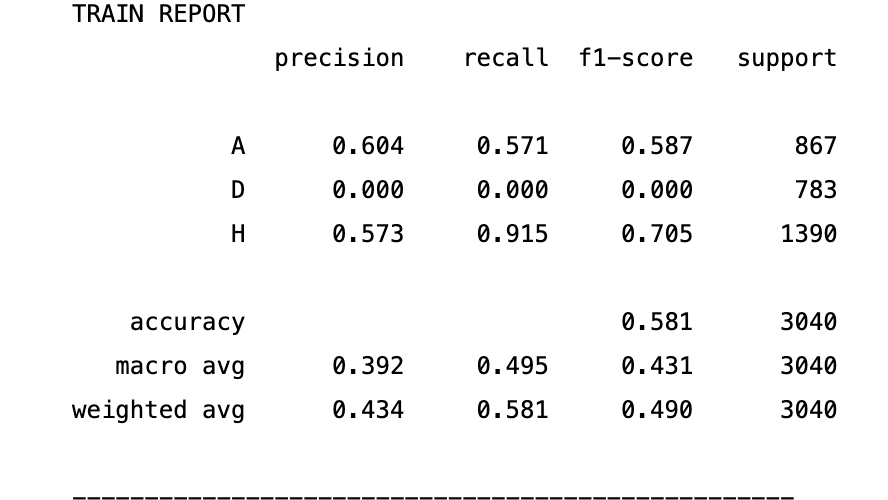
\includegraphics[scale=0.37]{tesina/img/lstm_concat/train_report.png}
%         \end{subcaptionblock}
%         \begin{subcaptionblock}{.5\textwidth}
%             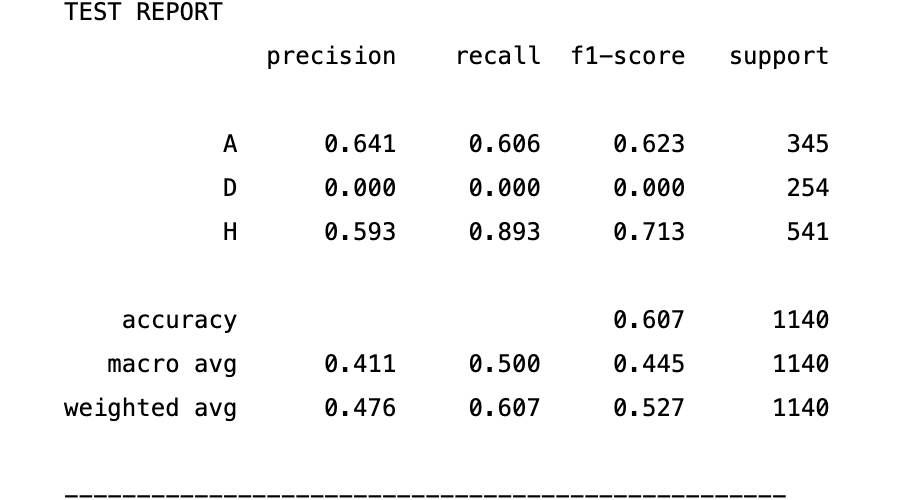
\includegraphics[scale=0.37]{tesina/img/lstm_concat/test_report.png}
%         \end{subcaptionblock}
%       \end{subcaptionblock}
%       \caption{LSTMconcat e prestazioni}
% \end{figure}

% \begin{figure}[h!]
%       \begin{subcaptionblock}{.55\textwidth}
%         \centering
%         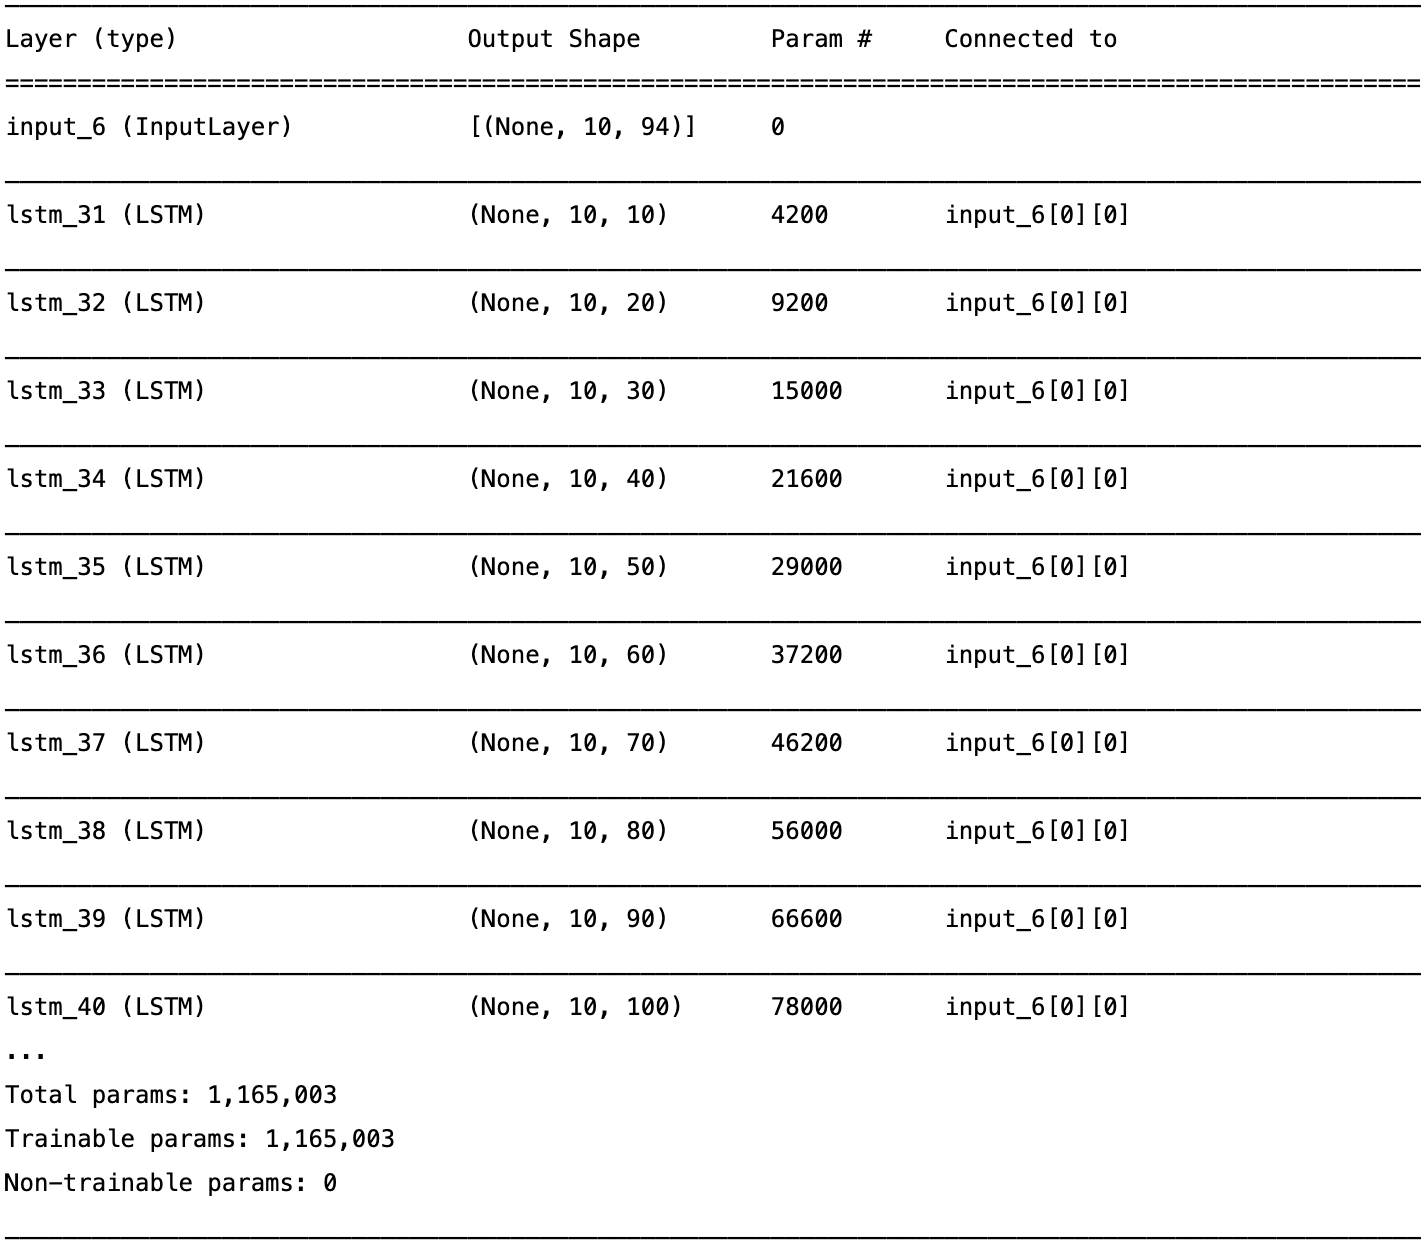
\includegraphics[scale=0.3]{tesina/img/lstm_parallelo/model_summary.png}
%       \end{subcaptionblock}
%       \begin{subcaptionblock}{.5\textwidth}
%         \begin{subcaptionblock}{.5\textwidth}
%             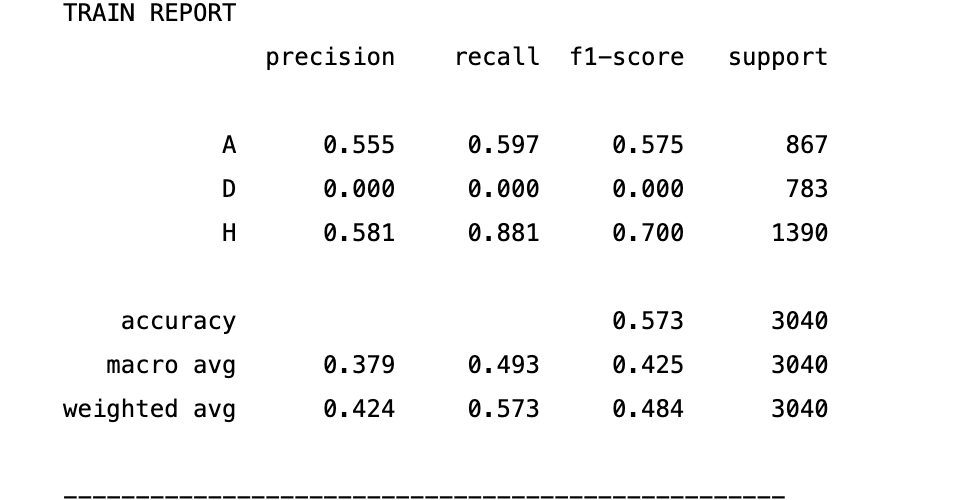
\includegraphics[scale=0.37]{tesina/img/lstm_parallelo/train_report.png}
%         \end{subcaptionblock}
%         \begin{subcaptionblock}{.5\textwidth}
%             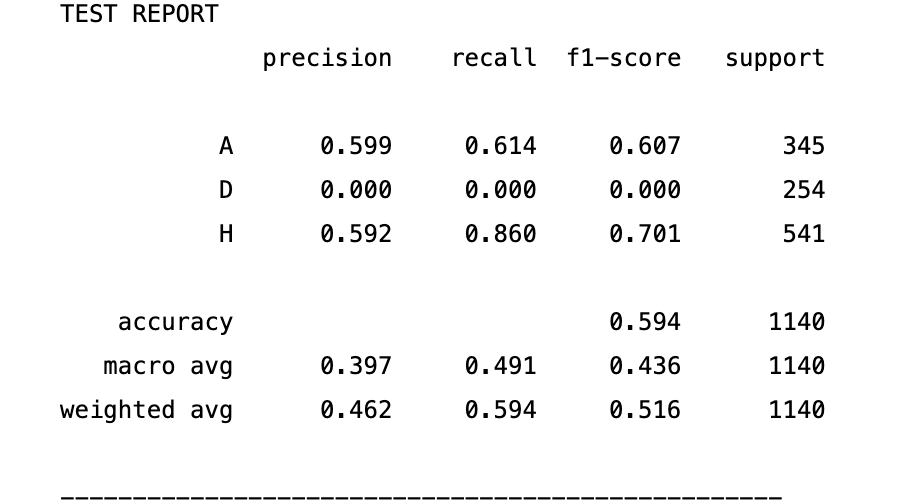
\includegraphics[scale=0.37]{tesina/img/lstm_parallelo/test_report.png}
%         \end{subcaptionblock}
%       \end{subcaptionblock}
%       \caption{LSTMparall e prestazioni}
% \end{figure}

\begin{lstlisting}[style=arch]
Model: "sequential_2"
_________________________________________________________________
Layer (type)                 Output Shape              Param #   
=================================================================
lstm_1 (LSTM)                (3040, 64)                16896     
_________________________________________________________________
flatten (Flatten)            (3040, 64)                0         
_________________________________________________________________
dense_6 (Dense)              (3040, 40)                2600      
_________________________________________________________________
dropout_6 (Dropout)          (3040, 40)                0         
_________________________________________________________________
dense_7 (Dense)              (3040, 20)                820       
_________________________________________________________________
dropout_7 (Dropout)          (3040, 20)                0         
_________________________________________________________________
dense_8 (Dense)              (3040, 10)                210       
_________________________________________________________________
dense_9 (Dense)              (3040, 3)                 33        
=================================================================
Total params: 20,559
Trainable params: 20,559
Non-trainable params: 0
_________________________________________________________________

\end{lstlisting}

\begin{lstlisting}[style=report]
TRAIN REPORT
                precision   recall  f1-score    support
            A       0.549    0.448     0.493        867
            D       0.000    0.000     0.000        783
            H       0.537    0.901     0.673       1390

     accuracy                          0.540       3040
    macro avg       0.363    0.450     0.389       3040
 weighted avg       0.402    0.540     0.448       3040
 __________________________________________________
TEST REPORT
                precision   recall  f1-score    support
            A       0.624    0.481     0.543        345
            D       0.000    0.000     0.000        254
            H       0.554    0.895     0.684        541

     accuracy                          0.570       1140
    macro avg       0.393    0.459     0.409       1140
 weighted avg       0.452    0.570     0.489       1140
\end{lstlisting}


\subsubsection*{GRU}
\begin{lstlisting}[style=arch]
Model: "sequential_3"
_________________________________________________________________
Layer (type)                 Output Shape              Param #   
=================================================================
gru (GRU)                    (3040, 22, 100)           30900     
_________________________________________________________________
dropout_8 (Dropout)          (3040, 22, 100)           0         
_________________________________________________________________
dense_10 (Dense)             (3040, 22, 1000)          101000    
_________________________________________________________________
dropout_9 (Dropout)          (3040, 22, 1000)          0         
_________________________________________________________________
dense_11 (Dense)             (3040, 22, 250)           250250    
_________________________________________________________________
dropout_10 (Dropout)         (3040, 22, 250)           0         
_________________________________________________________________
dense_12 (Dense)             (3040, 22, 3)             753       
=================================================================
Total params: 382,903
Trainable params: 382,903
Non-trainable params: 0
_________________________________________________________________

\end{lstlisting}

\begin{lstlisting}[style=report]
TRAIN REPORT
                precision   recall  f1-score    support
            A       0.621    0.611     0.616        867
            D       0.358    0.049     0.085        783
            H       0.610    0.913     0.731       1390

     accuracy                          0.604       3040
    macro avg       0.530    0.524     0.478       3040
 weighted avg       0.548    0.604     0.532       3040
 __________________________________________________
TEST REPORT
                precision   recall  f1-score    support
            A       0.585    0.591     0.588        345
            D       0.333    0.051     0.089        254
            H       0.604    0.839     0.702        541

     accuracy                          0.589       1140
    macro avg       0.507    0.494     0.460       1140
 weighted avg       0.538    0.589     0.531       1140
\end{lstlisting}


\subsubsection*{Bidirectional}
Di seguito viene mostrata l'architettura \textit{\textbf{Bidirectional}} utilizzata che, tuttavia, ha portato a pessime prestazioni, andando a \textit{overfittare} sui dati di training. Questo comportamento è motivato dalla poca coerenza tra gli approcci adottati e l'architettura in questione.
\begin{lstlisting}[style=arch]
Model: "sequential_4"
_________________________________________________________________
Layer (type)                 Output Shape              Param #   
=================================================================
bidirectional (Bidirectional (3040, 22, 128)           33792     
_________________________________________________________________
dropout_11 (Dropout)         (3040, 22, 128)           0         
_________________________________________________________________
dense_13 (Dense)             (3040, 22, 1000)          129000    
_________________________________________________________________
dropout_12 (Dropout)         (3040, 22, 1000)          0         
_________________________________________________________________
dense_14 (Dense)             (3040, 22, 250)           250250    
_________________________________________________________________
dropout_13 (Dropout)         (3040, 22, 250)           0         
_________________________________________________________________
dense_15 (Dense)             (3040, 22, 3)             753       
=================================================================
Total params: 413,795
Trainable params: 413,795
Non-trainable params: 0
_________________________________________________________________

\end{lstlisting}

\begin{lstlisting}[style=report]
TRAIN REPORT
                precision   recall  f1-score    support
            A       0.689    0.803     0.742        867
            D       0.762    0.420     0.542        783
            H       0.769    0.884     0.823       1390

     accuracy                          0.741       3040
    macro avg       0.740    0.702     0.702       3040
 weighted avg       0.744    0.741     0.727       3040
 __________________________________________________
TEST REPORT
                precision   recall  f1-score    support
            A       0.511    0.594     0.550        345
            D       0.269    0.126     0.172        254
            H       0.627    0.719     0.670        541

     accuracy                          0.549       1140
    macro avg       0.469    0.480     0.464       1140
 weighted avg       0.512    0.549     0.523       1140
\end{lstlisting}


\subsubsection*{WaveNet}
L'ultima architettura testata è la \textit{\textbf{WaveNet}}\cite{DBLP:journals/corr/OordDZSVGKSK16}, che ci ha permesso di introdurre layer convolutivi (a sostituzione di quelli ricorrenti), layer di \textit{\textbf{BatchNormalization}} e \textit{\textbf{Pooling}}, che precedono gli ultimi strati \textit{Fully Connected}.
\begin{lstlisting}[style=arch]
Model: "sequential"
_________________________________________________________________
Layer (type)                 Output Shape              Param #   
=================================================================
conv1d (Conv1D)              (3040, 94, 32)            96        
_________________________________________________________________
batch_normalization (BatchNo (3040, 94, 32)            128       
_________________________________________________________________
activation (Activation)      (3040, 94, 32)            0         
_________________________________________________________________
max_pooling1d (MaxPooling1D) (3040, 94, 32)            0         
_________________________________________________________________
conv1d_1 (Conv1D)            (3040, 94, 64)            4160      
_________________________________________________________________
batch_normalization_1 (Batch (3040, 94, 64)            256       
_________________________________________________________________
activation_1 (Activation)    (3040, 94, 64)            0         
_________________________________________________________________
max_pooling1d_1 (MaxPooling1 (3040, 94, 64)            0         
_________________________________________________________________
conv1d_2 (Conv1D)            (3040, 94, 256)           33024     
_________________________________________________________________
batch_normalization_2 (Batch (3040, 94, 256)           1024      
_________________________________________________________________
activation_2 (Activation)    (3040, 94, 256)           0         
_________________________________________________________________
max_pooling1d_2 (MaxPooling1 (3040, 94, 256)           0         
_________________________________________________________________
flatten (Flatten)            (3040, 24064)             0         
_________________________________________________________________
dense (Dense)                (3040, 100)               2406500   
_________________________________________________________________
dense_1 (Dense)              (3040, 3)                 303       
=================================================================
Total params: 2,445,491
Trainable params: 2,444,787
Non-trainable params: 704
_________________________________________________________________
\end{lstlisting}
\begin{lstlisting}[style=report]
TRAIN REPORT
              precision    recall  f1-score   support

           A      0.628     0.537     0.579       867
           D      0.499     0.249     0.332       783
           H      0.622     0.853     0.719      1390

    accuracy                          0.608      3040
   macro avg      0.583     0.547     0.544      3040
weighted avg      0.592     0.608     0.580      3040

--------------------------------------------------
TEST REPORT
              precision    recall  f1-score   support

           A      0.587     0.646     0.615       345
           D      0.286     0.102     0.151       254
           H      0.619     0.765     0.684       541

    accuracy                          0.582      1140
   macro avg      0.497     0.505     0.483      1140
weighted avg      0.535     0.582     0.544      1140

--------------------------------------------------  
\end{lstlisting}